\documentclass[letterpaper, 10pt, conference]{ieeeconf}
\IEEEoverridecommandlockouts \overrideIEEEmargins
\usepackage{amsmath,amssymb,url}
\usepackage{graphicx,subfigure,tikz}
\usepackage{color}
\newcommand{\argmax}{\operatornamewithlimits{argmax}}

\newcommand{\norm}[1]{\ensuremath{\left\| #1 \right\|}}
\newcommand{\bracket}[1]{\ensuremath{\left[ #1 \right]}}
\newcommand{\braces}[1]{\ensuremath{\left\{ #1 \right\}}}
\newcommand{\parenth}[1]{\ensuremath{\left( #1 \right)}}
\newcommand{\pair}[1]{\ensuremath{\langle #1 \rangle}}
\newcommand{\met}[1]{\ensuremath{\langle\langle #1 \rangle\rangle}}
\newcommand{\refeqn}[1]{(\ref{eqn:#1})}
\newcommand{\reffig}[1]{Fig. \ref{fig:#1}}
\newcommand{\tr}[1]{\mathrm{tr}\ensuremath{\negthickspace\bracket{#1}}}
\newcommand{\trs}[1]{\mathrm{tr}\ensuremath{[#1]}}
\newcommand{\ave}[1]{\mathrm{E}\ensuremath{[#1]}}
\newcommand{\deriv}[2]{\ensuremath{\frac{\partial #1}{\partial #2}}}
\newcommand{\SO}{\ensuremath{\mathsf{SO(3)}}}
\newcommand{\T}{\ensuremath{\mathsf{T}}}
\renewcommand{\L}{\ensuremath{\mathsf{L}}}
\newcommand{\so}{\ensuremath{\mathfrak{so}(3)}}
\newcommand{\SE}{\ensuremath{\mathsf{SE(3)}}}
\newcommand{\se}{\ensuremath{\mathfrak{se}(3)}}
\renewcommand{\Re}{\ensuremath{\mathbb{R}}}
\newcommand{\aSE}[2]{\ensuremath{\begin{bmatrix}#1&#2\\0&1\end{bmatrix}}}
\newcommand{\ase}[2]{\ensuremath{\begin{bmatrix}#1&#2\\0&0\end{bmatrix}}}
\newcommand{\D}{\ensuremath{\mathbf{D}}}
\renewcommand{\d}{\ensuremath{\mathfrak{d}}}
\newcommand{\Sph}{\ensuremath{\mathsf{S}}}
\renewcommand{\S}{\Sph}
\newcommand{\J}{\ensuremath{\mathbf{J}}}
\newcommand{\Ad}{\ensuremath{\mathrm{Ad}}}
\newcommand{\intp}{\ensuremath{\mathbf{i}}}
\newcommand{\extd}{\ensuremath{\mathbf{d}}}
\newcommand{\hor}{\ensuremath{\mathrm{hor}}}
\newcommand{\ver}{\ensuremath{\mathrm{ver}}}
\newcommand{\dyn}{\ensuremath{\mathrm{dyn}}}
\newcommand{\geo}{\ensuremath{\mathrm{geo}}}
\newcommand{\Q}{\ensuremath{\mathsf{Q}}}
\newcommand{\G}{\ensuremath{\mathsf{G}}}
\newcommand{\g}{\ensuremath{\mathfrak{g}}}
\newcommand{\Hess}{\ensuremath{\mathrm{Hess}}}
\newcommand\circled[1]{%
  \tikz[baseline=(C.base)]\node[draw,circle,inner sep=0.5pt](C) {#1};\!
}

\title{\LARGE \bf
%Recursive Kalman-Mahanobis JPDAF Minimization to avoid Coalescence of Estimates in Close Proximity
Optimal Joint Probabilistic Data Association Filter Avoiding Track Coalescence}
\author{Evan Kaufman and Taeyoung Lee
 \thanks{Evan Kaufman and Taeyoung Lee are with Department of Aerospace Engineering, George Washington University, Washington, DC. Email: {\tt\footnotesize \{evankaufman, tylee\}@gwu.edu }}
}

\newcommand{\EditTL}[1]{{\color{red}\protect #1}}
\renewcommand{\EditTL}[1]{{\protect #1}}

\newtheorem{definition}{Definition}
\newtheorem{lem}{Lemma}
\newtheorem{prop}{Proposition}
\newtheorem{remark}{Remark}


\begin{document}
\allowdisplaybreaks


\maketitle \thispagestyle{empty} \pagestyle{empty}

\begin{abstract}
We consider the tracking problem of two objects in close proximity where the measurement originations are unknown. The joint probabilistic data association filter (JPDAF) is useful for real-time applications because the measurement updates can be recursively and effectively applied based on the likelihood of association. However, when close neighboring tracks share measurements, the JPDAF tends to causes estimates to coalesce. Therefore we propose a Kalman-Mahalanobis minimizing JPDAF (KMMJPDAF) that chooses the gains of the measurement update to minimize both the posterior uncertainty and a measure of similarity based from the Mahalanobis distance. The algorithm is derived and explained, involving a higher computational cost that the JPDAF, but not high enough to prevent the possiblity real-time implementation. We discuss how to tune the parameters and when the algorithm is best used. Numerical simulations are used to evaluate the performance of the algorithms and conclusions are drawn on these results.
\end{abstract}

%_______________________________________________%

\section{Introduction}
Data association is a heavily studied field with many applications involving estimation involving measurements that are not necessarily originating from a single object.
We consider applications wherein multiple objects of interest enter the field of view of a sensor; however, the measurement origin is unknown.
To properly track these objects, we require estimation techniques to associate objects with measurements.
When the objects are in very close proximity, the association uncertainty grows, and an effective algorithm is necessary to maintain close estimations of the objects.

A variety of data association techniques with varying performance.
Some approaches such as multiple hypothesis tracking (MHT) and probability hypothesis density (PHD) techniques involve a high computational load, especially when objects are in close proximity, making real-time implementation more difficult~\cite{MHT1},~\cite{PHD1}~\cite{PHD2}.
Many other techniques may involve the Kalman filter (KF) or extended KF (EKF), which are well studied and provide a framework for recursive data association techniques that is much easier to implement in real-time.
A common heuristic approach is known as the nearest neighbor filter (NNF), which is a simple algorithm that only updates estimates for measurements with the closest square Mahalnobis distance, updating other objects only with their predictions~\cite{NN2}.
This is considered a \emph{hard decision} in~\cite{JPDAF1}, or that every measurement update receives full weighting; if the decision is incorrect, these measurement updates can result in detrimental effects to the associations of the estimates, so this technique is avoided in the analysis of this paper.
Alternatively, some approaches calculate the minimum mean square error (MMSE) of the estmates and their associated uncertainty.
The probabilistic data association (PDA) technique is effective in tracking a single object because it updates with a \emph{soft decision}; in particular, this approach updates provides a weighting from a likelihood of measurement association.

The joint PDA (JPDA) is an extension of the PDA to incorporate multiple objects~\cite{JPDAF1},~\cite{TrackDataAssoc}.
The JPDA filter (JPDAF) is particularly advantageous in multi-object scenarios because when objects share measurements, the soft decisions prevent loss of information, which occurs with hard decisions.
However, when neighboring objects share measurements, the estimates are subject to coalescence.

Some approaches to avoid track coalescence involve the concept that when the exact nearest neighbor probabilistic data association (ENNPDA) is applied, which associates a measurement with a strong decision to the most likely estimate, the estimates are insensitive to track coalescence [Blom 2000].
By pruning the tracks, or designing a set of rules to determine high likelihood scenarios, a weighing scheme is applied to the measurement updates.
For example in [Fitzgerald], the algorithm involves a set of rules based on the data received with respect to the estimates.
A special logic is introduced that determines how weighting of the updates is defined or if a new track should be considered.
In some cases, an incorrectly associated estimate measurement may receive full weighting in the update.
Other criteria for choosing hard and soft decisions to avoid track coalescence are detailed in~\cite{Coal_d} and~\cite{Coal_e}, which may be effective, but are rather heuristic by nature and risk assigning an incorrect hard decision.
Some other approaches involve coupling joint states. Explain more and validate last citation...

We propose a novel approach to removing coalescence by minimizing a similarity index of the estimates.
Instead of choosing a different means of weighting the measurement updates or coupling their distributions, we design an optimal recursive estimation algorithm that chooses gains to compensate for the effects of coalescence.
The algorithm derived in this paper can be applied in real-time without the heuristic nature, coupling, or the risk of hard decisions from the current coalescence avoidance approaches.

The paper is organized as follows: the problem is formally presented in Section \ref{ProbDef}.
The optimal gain derivation and algorithm description is presented in Section \ref{KMM}.
We discuss how to implement the algorithm and how to appropriately weight the minimized cost function in section \ref{AlgImpTuning}.
We consider a satellite tracking example of this technique in Section \ref{NumRes}.
Finally, we discuss results and applications for the KMMJPDAF in Section \ref{ConclusionFutureWork}.

%A considerable amount of work has been done to solve the data association problem. Approaches vary in their performance, including the portion of correct associations, the ability to maintain the correct tracks, and the computational cost. In this section, we examine some of the current techniques with respect to tracking two objects in close proximity and propose a new approach to solve this problem.
%
%The multiple hypothesis tracking (MHT) approach considers multiple hypotheses for how the data may be associated for multiple tracks~\cite{MHT1}. As new information becomes available, hypotheses are evaluated, in some cases removed, and predicted again. However in complicated problems, the number hypothesis may explode. One approach to remove this issue from the close proximity problem is known as track pruning, where incompatible tracks are highlighted and only the most likely tracks are considered. This approach is complex and involves a high computational cost, so implementing this approach in real-time is very difficult. Furthermore according to~\cite{PHD1}, MHT is subject to poor results with objects in close proximity.
%
%The probability hypothesis density (PHD) process is a propagation of the first moment of a joint distribution~\cite{PHD2}. A typical PHD considers a sub-area of interest where peaks from the integral of the PHD are considered objects. In many cases, the PHD filter is hindered by computational complexity, growing exponentially with the number of objects and further increasing when the possibility that objects may enter or leave the sub-area considered. An approach described in~\cite{PHD1} maintains a tracker for each object of interest. Each tracker accounts for a priori estimates of state and dynamics to predict the probability densities for the next time step. The process is complex and involves separating the sub-spaces into cells wherein likelihoods of each object are used to define peaks and dummy peaks, where a single track or multiple tracks exist, respectively. This approach can be more computationally expensive than other recursive approaches as the algorithm is among the most complex and the resolution (defined by size of the cells where peaks lie) will require modification as objects become close.
%
%The nearest neighbor filter (NNF) is a heuristic approach that calculates the magnitude between the measurement and its prediction~\cite{JPDAF1}; the state with smallest square Mahalanobis distance of the innovation and its covariance receives a filtered update with the measurement while all other states of interest are updated with only their predictions~\cite{NN2}; this is referred to as a \emph{hard decision}~\cite{JPDAF1}. This approach adds a simple step to the EKF at the cost of accuracy as the probability of association is not explicitly calculated.
%
%The JPDAF is an extension of the probabilistic data association filter (PDAF) described in~\cite{JPDAF1} and~\cite{TrackDataAssoc}, which calculates the probabilities that measurements belong to an individual estimate. The JPDAF is designed to track multiple objects of interest. The estimates are updated with a \emph{soft decision}, or by a weighting factor based from the probability of association. However, when more than one object of interest share measurements, the objects are subject to a measurement updates that draw the estimates together, or coalesce the estimates.
%
%There are a few approaches to remove coalescence from the JPDAF. Much like the MHT, some approaches iinvolve track pruning and are detailed in~\cite{Coal1},~\cite{Coal2},~\cite{Coal_d}, and~\cite{Coal_e}, but this is computationally complex and can suffer when implementing the approach recursively. Other techniques such as those described in~\cite{Coal_c},~\cite{Coal_g},~\cite{Coal_i}, and~\cite{Coal_j} involve assigning hard decisions. The criteria and performance of these techniques vary, but each eliminate coalescence by never sharing a measurement, which can yield fully weighted incorrect associations that may cause detrimental effects such as estimates switching trajectories of crossing tracks. To decrease this problem, an arbitrary scaling factor is applied in~\cite{Coal_f} wherein the more likely association is given more weight as the less likely association weightings are decreased, yielding a hybrid technique between the NNF and the JPDAF. This approach may yield improved results with a heuristic weighting scheme but results vary with the application and expected data.
%
%Therefore, we propose a systematic approach that minimizes a weighted cost of uncertainty and similarity. We design the KMMJPDAF to minimize the posterior uncertainty much like the Kalman filter in addition to evaluating the Mahalanobis distance involved with updating the states. The paper is organized as follows: the problem is formally presented in Section \ref{ProbDef}. The optimal gain derivation and algorithm description is presented in Section \ref{KMM}. We discuss how to implement the algorithm and how to appropriately weight the minimized cost function in section \ref{AlgImpTuning}. We consider a satellite tracking example of this technique in Section \ref{NumRes}. Finally, we discuss results and applications for the KMMJPDAF in Section \ref{ConclusionFutureWork}.

%_______________________________________________%

\section{Problem Definition}
\label{ProbDef}
The objects of interest are assumed to have nonlinear dynamics and each have Gaussian distributed estimates. We evaluate objects at time $k$ and linearize the system dynamics with respect to time $k-1$. We define the JPDAF algorithm such that we update the state as measurements are received, i.e. we only consider a single measurement rather than a scan of measurements. Furthermore, this research is concerned with the two estimates in very close proximity; hence we assume that the measurement originations are from a single object of interest and not from other sources of clutter.

\subsection{Time Update} We denote an estimate of state with a $\hat{.}$, and the estimates before and after the measurement update with a $.^-$ and $.^+$, respectively. We define $x\in \Re^{n\times1}$ as the state vector and $P\in\Re^{n\times n}$ as its covariance. The time update provides the predicted state and covariance
\begin{gather}
\hat{x}_{k}^{-}=A_{k-1}\hat{x}_{k-1} \\
P_{k}^{-}=A_{k-1}P_{k-1}A_{k-1}^T+Q_k.
\end{gather}
The covariance of process noise is captured in $Q_k$ and no control input is considered.

\subsection{Measurement Update} The measurement update requires an innovation
\begin{equation}
\label{innovation}
e_{k}=z_{k}-\hat z_{k|k-1}
\end{equation}
where $z_{k}\in\Re^{m\times1}$ is the measurement received and measurement prediction $\hat z_{k|k-1}=H_{k}\hat{x}_{k}^{-}$; $H_{k}$ maps $\hat{x}_{k}^{-}$ from the state space to the measurement space.% Check this line terminology
We simplify the equations for probability of association from~\cite{JPDAF1} and~\cite{TrackDataAssoc} to include only a single measurement that always belongs to either one of the two objects considered; hence the process of association is limited two mutually exclusive scenarios: we measure object 1 and not object 2 or we measure object 2 and not object 1. After some manipulation we can show for object $t$, the relative probability $\beta_t$ is simplified to
\begin{gather}
\beta_t=\frac{f_t}{\displaystyle\sum\limits_{\tau=1}^2 f_{\tau}} \\
f_t=\mathcal{N}[z_{k};\hat z_{k|k-1},S].
\end{gather}
The innovation covariance $S$ is defined as
\begin{equation}
S_k=H_{k}P_{k}^{-}H_{k}^T+R_k
\end{equation}
where $R_k$ is the covariance of the measurement. The gain to minimize the posterior uncertainty with cost function $J_P=\tr{P_{k+1}^{+}}$ is equivalent to the Kalman gain
\begin{equation}
\label{KalmanGain}
K_{k}=P_{k}^{-}H_{k}^TS_k^{-1}
\end{equation}
which is used to calculate the updated state and its covariance for each estimate
\begin{gather}
\label{xhatp}
\hat{x}_{k}^{+}=\hat{x}_{k}^{-}+\beta K_{k}e_{k} \\
\label{oldPp}
P_{k}^{+}=P^-_{k}-\beta K_{k}S_kK_{k}^{T}
\end{gather}
for the JPDAF, but not for the KMMJPDAF. For the KMMJPDAF we derive a new gain which is not compatible with Equation \ref{oldPp}, which is a manipulation involving Equation \ref{KalmanGain} of the original form (ignoring the $\beta$ term)
\begin{equation}
\label{genPp}
P_{k}^{+}=(I-K_{k}H_{k})P_{k}^{-}(I-K_{k}H_{k})^T+K_{k}R_kK_{k}^T
\end{equation}
from ~\cite{OptEst1}. Hence in order to properly update the posterior covariance when we include coalescence into the minimization, we manipulate Equation \ref{genPp} to involve relative weighting $\beta$ of the measurement update. Note that time step subscripts will be assumed at $k$ from here forward for simplicity. Obtaining a gain accounting for posterior uncertainty and coalescence takes the generalized form
\begin{equation}
\label{newPp}
P^+=P^--\beta[KHP^-+P^-H^TK^T-K(HP^-H^T+R)K^T].
\end{equation}
Note that if we insert the Kalman gain from Equation \ref{KalmanGain} into Equation \ref{newPp}, we can manipulate the result to Equation \ref{oldPp}.

%_______________________________________________%

\section{Kalman-Mahalanobis Optimization}
\label{KMM}
We derive the gain of the measurement update for object $t$ to minimize a weighted sum of the uncertainty and a similarity measure
\begin{equation} \label{CostDef}
J=J_P+cJ_S
\end{equation}
where $J_P$ is the cost associated with the posterior state covariance, $J_S$ is the cost associated with the similarity of the two distributions, and $c$ is a positive scalar constant for relative weighting. The following equations in this section will focus on object 1 but the derivations with respect to object 2 are indentical except with subscripts switched.

\subsection{Uncertainty Cost} The derivation of $J_P$ is a fairly straightforward adaptation of the Kalman filter from~\cite{OptEst1} with the included JPDAF weighting. Evaluating the trace of Equation \ref{newPp} for object 1,
\begin{align}
\begin{split}
J_{P,1}=&\tr{P_1^+} \\
=& \tr{P_1^-}+\beta_1(\tr{K_1(H_1P_1^-H_1^T+R_1)K_1^T}\\
&-2\tr{K_1H_1P_1^-}).
\end{split}
\end{align}
We can take its derivative $\frac{\partial J_{P,1}}{\partial K_{1}}$ using the property $\frac{\partial}{\partial X}\tr{XYX^T}=2XY$ for symmetric $Y$ to obtain
\begin{align}
\label{CostP}
\begin{split}
\frac{\partial J_{P,1}}{\partial K_{1}}&=2\beta_1\{{K_1(H_1P_1^-H_1^T+R_1)-P_1^-H_1^T}\}.
\end{split}
\end{align}

 \subsection{Similarity Cost} We choose the Mahalanobis distance to measure similarity because it yields a scalar result and taking its derivative with respect to measurement update gains is possible. We use $P_1^-$ as the covariace estimation of object 1 for the Mahalanobis distance with respect to the estimated mean of object $2$ can take the form
\begin{align}
\label{M1}
M_1=u_1^{\frac{1}{2}}
\end{align}
where
\begin{align} \label{u_1}
\begin{split}
u_1=&(\hat x_1^+-\hat x_2^+)^{T}{P_1^-}^{-1}(\hat x_1^+-\hat x_2^+)\\
=&\{\hat x_1^{-T}{P_1^-}^{-1}\hat x_1^-
-2\hat x_1^{-T}{P_1^-}^{-1}\hat x_2^-\\
&+2\beta_1(\hat x_1^{-}-\hat x_2^{-})^T{P_1^-}^{-1}K_1e_1
+\hat x_2^{-T}{P_1^-}^{-1}\hat x_2^-\\
&+2\beta_2(\hat x_2^{-}-\hat x_1^{-})^T{P_1^-}^{-1}K_2e_2
+\beta_1^2e_1^TK_1^T{P_1^-}^{-1}K_1e_1\\
&-2\beta_1\beta_2e_2^TK_2^T{P_1^-}^{-1}K_1e_1+\beta_2^2e_2^TK_2^T{P_1^-}^{-1}K_2e_2\}
\end{split}
\end{align}
which is the most reduced form to differentiate with respect to $K_1$ and $K_2$. However, the Mahalanobis distance is an increasing measure as similarity decreases. Therefore we wish to minimize $M_1^{-2a}$ for $a>0$. Furthermore as the Mahalanobis distance is a scalar quantity, we can use the property $\frac{\partial g(u_1)}{\partial K_1}=\frac{\partial g(u_1)}{\partial u_1}\frac{\partial u_1}{\partial K_1}$ such that $J_{C,1}=M_1^{-2a}=g(u_1)=u_1^{-a}$. We take the derivative of the similarity measure using $u_1=f(K_1,K_2)$ from Equations \ref{M1} and \ref{u_1} as well as the properties $\frac{\partial}{\partial X} \tr{AXB}=A^TB^T$ and $\frac{\partial}{\partial X}\tr{AXBX^TC}=A^TC^TXB^T+CAXB$ to obtain, after some manipulation,
\begin{align}
\begin{split}
\label{CostS}
\frac{\partial J_{S,1}}{\partial K_1}=&-au_1^{-(a+1)}\frac{\partial u}{\partial K_1}\\
=&2a\beta_1u_1^{-(a+1)}\{
{P_1^-}^{-1}(\hat x_2^--\hat x_1^-)\\
&-\beta_1{P_1^-}^{-1}K_1e_1
+\beta_2{P_1^-}^{-1}K_2e_2
\}e_1^T.
\end{split}
\end{align}

We absorb the constants from Equations \ref{CostP} and \ref{CostS} into $c$ from Equation \ref{CostDef} and use a nonlinear equation solver for the optimal gains $K_1$ and $K_2$ in the joint equations
\begin{align}
\label{Opt1}
\begin{split}
\frac{\partial J_{1}}{\partial K_{1}}=&K_1(H_1P_1^-H_1^T+R_1)-P_1^-H_1^T\\
&+cu_1^{-(a+1)}\{
{P_1^-}^{-1}(\hat x_2^--\hat x_1^-)\\
&-\beta_1{P_1^-}^{-1}K_1e_1
+\beta_2{P_1^-}^{-1}K_2e_2
\}e_1^T\\
=&0_{n\times m}
\end{split}
\end{align}
and similarly
\begin{align}
\label{Opt2}
\begin{split}
\frac{\partial J_{2}}{\partial K_{2}}=&K_2(H_2P_2^-H_2^T+R_2)-P_2^-H_2^T\\
&+cu_2^{-(a+1)}\{
{P_2^-}^{-1}(\hat x_1^--\hat x_2^-)\\
&-\beta_2{P_2^-}^{-1}K_2e_2
+\beta_1{P_2^-}^{-1}K_1e_1
\}e_2^T\\
=&0_{n\times m}.
\end{split}
\end{align}
These equations vary in computational cost depending on the level of precision of the nonlinear equation solver. Note that ${P_1^-}^{-1}$ and ${P_2^-}^{-1}$ are symmetric inverses and must only be calculated once each.

%_______________________________________________%

\section{Algorithm Implementation and Tuning}
\label{AlgImpTuning}
This algorithm requires considerably more computational cost than the JPDAF alone; hence, we only implement this algorithm when the likelihood of coalescence is high. For example, if the association of a measurement belongs primarily to a single estimate, the KMMJPDAF and JPDAF yield similar results so we choose JPDAF because of its closed form solution and hence lower computational cost. Therefore depending on the application, we determine thresholds such that beyond some spacing between the a priori estimates we default to the JPDAF algorithm for speed.

We must also examine the shape of the cost function. Consider Figure \ref{CostTrends}, which contains a variation of a single element of $K_1$ from an example in Section \ref{NumRes} and plots both cost functions of object 1. The uncertainty cost minimizes at a single point. However, the similarity cost contains a maximum. If we incorrectly choose $K_1$ and $K_2$ to maximize $J_S$, this would serve to increase coalescence because similarity would be increasing at a maximum rate due only to a measurement update.

\begin{figure}
\centerline{
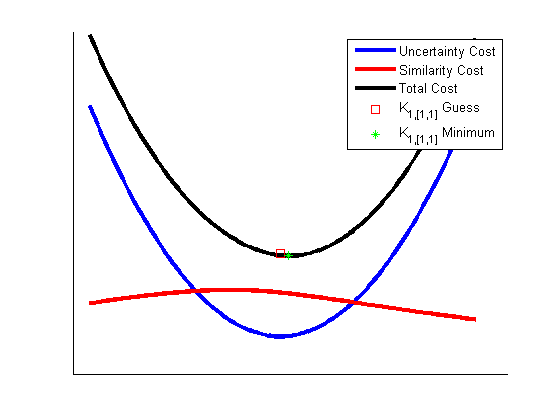
\includegraphics[width=9cm]{CostTrends.png}
	}
\caption{The cost functions of object 1 ($J_{P,1}$, $cJ_{C,1}$, and $J_{1}$) are examined under the variation of a single element of $K_1$. The resulting cost function (black) is minimized slightly to the left of the uncertainty cost function (blue). In Kalman filtering applications, including the JPDAF, only the uncertainty cost function is minimized.}
\label{CostTrends}
\end{figure}

There are a few approaches to avoid this detrimental scenario. First, we can choose $a$ and $c$ properly. Decreasing $a$ serves to amplify and flatten out $J_S$. Once a desired cost function shape as achieved, we can choose $c$ to bring $J_S$ to an appropriate scaling. In practice, the JPDAF is a very effective algorithm for estimation of multiple objects, which only relies on $J_P$, so $J_S$ is chosen to be very small in comparison only to remove coalescence from the estimates (Figure \ref{CostTrends} shows $cJ_{S,1}$ much larger in magnitude than in practice for illustration). Choice of these parameters leads to trade-offs: if $a$ is decreased along with $c$, the similarity cost varies less, decreasing the beneficial effects of the KMMJPDAF over the JPDAF. However, when $a$ is increased (and $c$ is increased to compensate), we may incorrectly solve for the similarity maximizing point.

We explore two techniques to find an effective minimization. First, we choose the initial guess of $K_1$ and $K_2$ to be that of the EKF, which is already located near the minimized point of uncertainty. Secondly, we only implement the KMMJPDAF when the a priori estimates are sufficiently spaced apart. This way we can maintain the desirable shape of the cost function and implement the KMMJPDAF for the majority of the region where coalescence poses an issue. Therefore, we have both minimum and maximum estimate spacing thresholds for which KMMJPDAF is appropriate.

%_______________________________________________%

\section{Numerical Results}
\label{NumRes}
We present a satellite tracking example where some parameters are varied to evaluate the performance of the KMMJPDAF with the JPDAF. We consider the scenario when we observe two satellites in LEO with crossing trajectories wherein we receive range measurements of unknown origination. For simplicity, both orbits occupy the same plane, so cylindrical coordinates are used to define our state variable $x=\begin{bmatrix} r & \dot r & \theta & \dot \theta\end{bmatrix}^{T}$. We only consider gravity, so we linearize the equations of motion and bring to the appropriate form
\begin{align}
A_{k-1}=
exp\left(\begin{bmatrix}
0 & 1 & 0 & 0 \\
\frac{2\mu}{r^3} +\dot{\theta}^2 & 0 & 0 & 2r\dot{\theta} \\
0 & 0 & 0 & 1 \\
2r^{-2}\dot{r}\dot{\theta} & -2r^{-1}\dot{\theta} & 0 &  -2r^{-1}\dot{r}\\
\end{bmatrix}dt\right)
\end{align}
where $\mu=GM_{Earth}=3.986\times10^5 km^3/s^2$ and $H=\begin{bmatrix} 1 & 0 & 0 & 0\end{bmatrix}$. We assume identical dynamics of the satellites (although this is not a requirement). We assume we have a priori knowlege from other measurement devices that provide an estimate of the state and covariance shortly before the two trajectories cross paths near $7000km$ from the center of the earth. We provide identical noisy range measurements to both the JPDAF and the KMMJPDAF algorithms. For the KMMJPDAF, we choose $a=0.01$ and $c=3\times10^{-8}$. We propagate the nonlinear equations of motion using \emph{ode45} in Matlab, and produce a measurement update every $0.1sec$ with an equal likelihood that its origination is from either object. For the results below, we refer to the KMMJPDAF algorithm as the KMMJPDAF when $0.05km\leq\norm{\hat z_1-\hat z_2}\leq0.4km$ and the JPDAF elsewhere due to the observations discussed in Section \ref{AlgImpTuning}.

\begin{figure}
\centerline{
	\subfigure[JPDAF]{\hspace*{0.07\textwidth}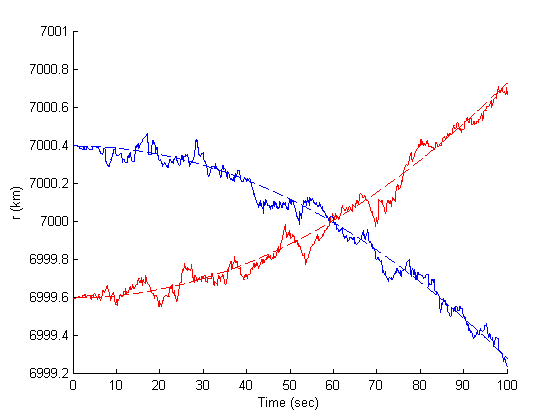
\includegraphics[width=9cm]{Case1JPDAF.png}\hspace*{0.07\textwidth}}
	}
\centerline{
	\subfigure[KMMJPDAF]{\hspace*{0.07\textwidth}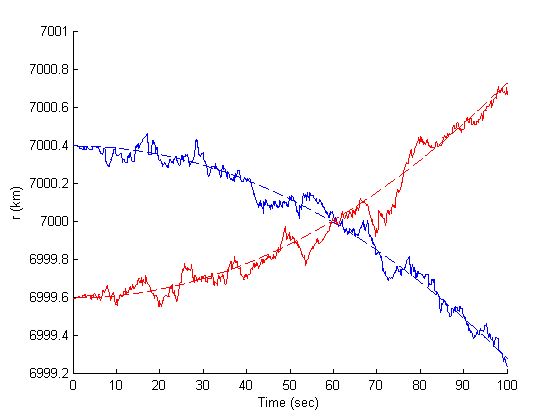
\includegraphics[width=9cm]{Case1KMMJPDAF.png}\hspace*{0.05\textwidth}}
	}
\caption{The estimation of object 1 (solid blue) is overlaid with the true trajectory of object 1 (dashed blue) and the estimation of object 2 (solid red) is overlaid with the true trajectory of object 2 (dashed red). When the JPDAF is able to properly track the trajectories, the KMMJPDAF yields similar results.}	
\label{Case1}
\end{figure}

The first results (Figure \ref{Case1}) shows a result wherein both algorithms are able to maintain the correct tracks. In fact, the results are very similar with two noteworthy differences. The first is that within $10 sec$ of crossing ($101$ measurements), the number of incorrect associated (weighted less than $50\%$ likelihood of association) for the JPDAF was $64$ whereas for the KMMJPDAF the number was $58$, but this is a minor difference in the metric. The second difference is that the JPDAF completed in $4.212sec$ while the KMMJPDAF ran in $6.8952sec$ on the same computer. For real-time implementation, either algorithm is capable of receiving these simple range measurements as described above, but when measurements are more complicated or are received at a faster rate, there can be cases where the performance of the JPDAF computational time makes the KMMJPDAF an inferior algorithm.

\begin{figure}
\centerline{
	\subfigure[JPDAF]{\hspace*{0.07\textwidth}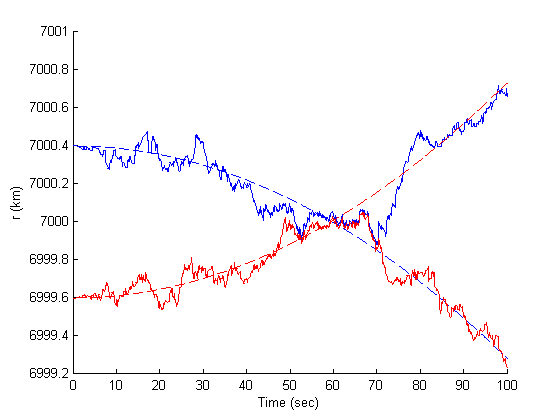
\includegraphics[width=9cm]{Case2JPDAF.png}\hspace*{0.07\textwidth}}
	}
\centerline{
	\subfigure[KMMJPDAF]{\hspace*{0.07\textwidth}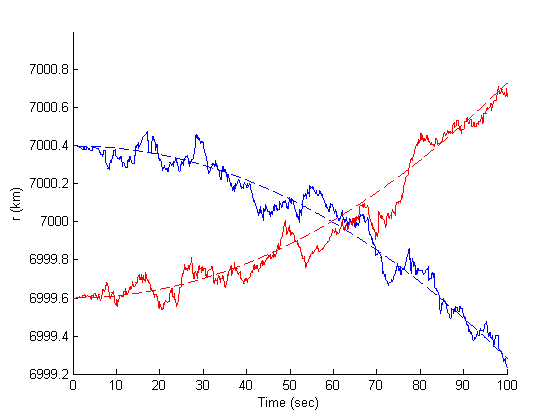
\includegraphics[width=9cm]{Case2KMMJPDAF.png}\hspace*{0.05\textwidth}}
	}
\caption{The JPDAF is subject to coalescence of the neighboring track, causing the estimations to switch trajectories. The KMMJPDAF is subject to less coalescence and hence does not exhibit this problem. Refer to Figure \ref{Case1} for the legend.}
\label{Case2}
\end{figure}

The noise of the measurements are increased in second example (Figure \ref{Case2}), and this causes the JPDAF to permanently lose the correct association after the crossing. The optimization of the KMMJPDAF compensates for the coalescence of the tracks, and hence correct track maintenance is achieved properly with this algorithm. The result of this example does not imply that the KMMJPDAF is impervious the the effects of coalescence; rather including similarity in the minimization serves to remove some of the coalescence from measurement updates. For the case presented here, choosing the KMMJPDAF rather than the JPDAF increases the computational time from $4.1964sec$ to $6.8018sec$ to maintain the estimates with the correct trajectories.

\begin{figure}
\centerline{
	\subfigure[Parameter change: $a=1$]{\hspace*{0.07\textwidth}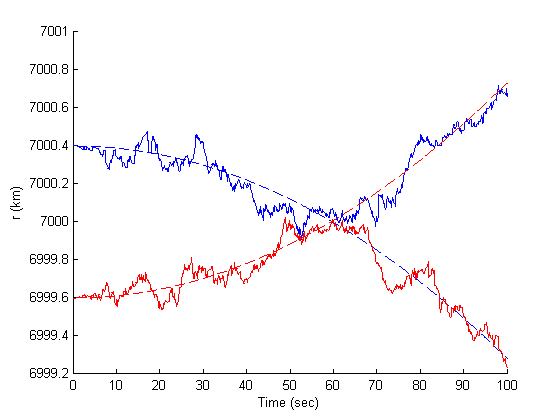
\includegraphics[width=9cm]{a1.png}\hspace*{0.07\textwidth}}
	}
\centerline{
	\subfigure[Parameter change: $c=1\times10^{-7}$]{\hspace*{0.07\textwidth}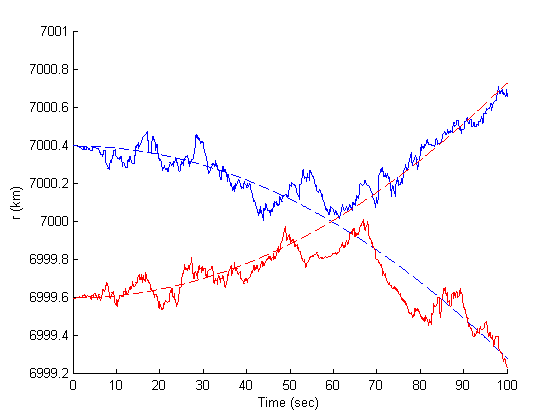
\includegraphics[width=9cm]{c1e7.png}\hspace*{0.05\textwidth}}
	}
\caption{These results show detrimental effects of choosing $a$ too great, attenuating the similarity cost function, yielding numerical results wherein coalescence causes poor estimation or choosing $c$ too great, increasing the similarity cost so much that the estimates diverge before they can ever cross. Refer to Figure \ref{Case1} for the legend.}
\label{changeParameters}
\end{figure}

We now use the last example to demonstrate the importance of choosing the parameters correctly for the effective implementation of the KMMJPDAF. In Figure \ref{changeParameters}.(a), we increase $a$ such that $a=1$, which serves to attenuate the similarity cost function. As a result, the gains are chosen to minimize uncertainty with greater weight much like the JPDAF. This results in increasing coalescence, yielding a poorer estimation of the states. In this case, the estimates are drawn very close together and diverge incorrectly.

We consider the same example but this time increase $c$ such that $c=1\times10^{-7}$, shown in Figure \ref{changeParameters}.(b). Increasing $c$ increases the similarity cost function proportionally according to Equation \ref{CostDef}. Contrary to the last example, the gains are chosen to decrease similarity of the estimates so much that the measurement updates serve to separate the estimates when the estimates become close. We experience the opposite effect with increasing $c$ than increasing $a$, but choosing either parameter poorly can lead to estimates switching trajectories.

%_______________________________________________%

\section{Conclusions and Future Work}
\label{ConclusionFutureWork}
We explore a new approach to removing coalescence by choosing measurement update gains that minimize with respect to similarity in addition to posterior uncertainty. The Mahalanobis distance is chosen as the measure of similarity because of its simple form and scalar result. We take the derivative of the similarity cost for both estimates, yielding a result with no closed form solution, but involving expressions with low computational cost that can be solved with a nonlinear equation solver. We discuss the importance of initial prediction for gains as well as thresholds for which the KMMJPDAF is appropriate.

We validate the theory with numerical simulations of a satellite tracking problem. We observe that if the JPDAF can properly handle tracking the objects of interest, this algorithm should be used due to its low computational cost. However, we show an example where the coalescence of the JPDAF causes the estimates to switch to incorrect trajectories. The KMMJPDAF is more robust to this issue and the estimates maintain their correct trajectories in the example. These results are only valid if the parameters of the cost function are chosen well; decreasing or increasing the similarity cost has the effect of coalescing or repelling the estimates, respectively, which can cause the estimates to lose the correct trajectories.

The KMMJPDAF can be extended to a variety of multi-object tracking applications when objects share measurements due to close proximity. One example, very close to that presented in Section \ref{NumRes}, is keeping logs of satellites using phased-array radar systems. In cases where satellites have similar measurement predictions over long periods of time, satellite tracking becomes much more difficult. Implementing a simple JPDAF can serve to coalesce the estimates, which can cause the estimates of the satellites to switch trajectories as shown in this paper. Therefore, including the KMMJPDAF under certain proximitiy conditions can expand our ability to track satellites. The KMMJPDAF has tracking applications for space, aerial, and underwater vehicles in close proximity and identification of individual agents in multi-agent systems.

Much like the Kalman filter, the KMMJPDAF can be effective for systems with well-known Gaussian distributions of state, sensor noise, and process. This paper has assumed that measurements come from a single object of interest at a single time and not clutter. Future work may involve expanding the capabilities of the algorithm. We can consider the measurements as a scan, or so that multiple measurements, including those from external sources of clutter, may belong to multiple objects at any timestep as a JPDAF does without the assumptions of this paper. A general form of this algorithm could be derived for these conditions.

Furthermore we can explore other techniques to measure similarity. The Mahanobis distance assumes the covariances of the estimates are close, which is not always accurate in all applications. Furthermore, we approximate the covariance in the Mahanobis distance with the a priori covariance, which changes with the measurement update. Hence, there are a few directions to improve the measure of posterior similarity.


\bibliography{BibMaster}
\bibliographystyle{IEEEtran}

\end{document}


